\documentclass[]{book}
\usepackage{lmodern}
\usepackage{amssymb,amsmath}
\usepackage{ifxetex,ifluatex}
\usepackage{fixltx2e} % provides \textsubscript
\ifnum 0\ifxetex 1\fi\ifluatex 1\fi=0 % if pdftex
  \usepackage[T1]{fontenc}
  \usepackage[utf8]{inputenc}
\else % if luatex or xelatex
  \ifxetex
    \usepackage{mathspec}
  \else
    \usepackage{fontspec}
  \fi
  \defaultfontfeatures{Ligatures=TeX,Scale=MatchLowercase}
\fi
% use upquote if available, for straight quotes in verbatim environments
\IfFileExists{upquote.sty}{\usepackage{upquote}}{}
% use microtype if available
\IfFileExists{microtype.sty}{%
\usepackage{microtype}
\UseMicrotypeSet[protrusion]{basicmath} % disable protrusion for tt fonts
}{}
\usepackage[margin=1in]{geometry}
\usepackage{hyperref}
\hypersetup{unicode=true,
            pdftitle={Using R for Introduction to Econometrics},
            pdfauthor={Christoph Hanck, Martin Arnold, Alexander Gerber and Martin Schmelzer},
            pdfborder={0 0 0},
            breaklinks=true}
\urlstyle{same}  % don't use monospace font for urls
\usepackage{natbib}
\bibliographystyle{apalike}
\usepackage{color}
\usepackage{fancyvrb}
\newcommand{\VerbBar}{|}
\newcommand{\VERB}{\Verb[commandchars=\\\{\}]}
\DefineVerbatimEnvironment{Highlighting}{Verbatim}{commandchars=\\\{\}}
% Add ',fontsize=\small' for more characters per line
\usepackage{framed}
\definecolor{shadecolor}{RGB}{248,248,248}
\newenvironment{Shaded}{\begin{snugshade}}{\end{snugshade}}
\newcommand{\KeywordTok}[1]{\textcolor[rgb]{0.13,0.29,0.53}{\textbf{#1}}}
\newcommand{\DataTypeTok}[1]{\textcolor[rgb]{0.13,0.29,0.53}{#1}}
\newcommand{\DecValTok}[1]{\textcolor[rgb]{0.00,0.00,0.81}{#1}}
\newcommand{\BaseNTok}[1]{\textcolor[rgb]{0.00,0.00,0.81}{#1}}
\newcommand{\FloatTok}[1]{\textcolor[rgb]{0.00,0.00,0.81}{#1}}
\newcommand{\ConstantTok}[1]{\textcolor[rgb]{0.00,0.00,0.00}{#1}}
\newcommand{\CharTok}[1]{\textcolor[rgb]{0.31,0.60,0.02}{#1}}
\newcommand{\SpecialCharTok}[1]{\textcolor[rgb]{0.00,0.00,0.00}{#1}}
\newcommand{\StringTok}[1]{\textcolor[rgb]{0.31,0.60,0.02}{#1}}
\newcommand{\VerbatimStringTok}[1]{\textcolor[rgb]{0.31,0.60,0.02}{#1}}
\newcommand{\SpecialStringTok}[1]{\textcolor[rgb]{0.31,0.60,0.02}{#1}}
\newcommand{\ImportTok}[1]{#1}
\newcommand{\CommentTok}[1]{\textcolor[rgb]{0.56,0.35,0.01}{\textit{#1}}}
\newcommand{\DocumentationTok}[1]{\textcolor[rgb]{0.56,0.35,0.01}{\textbf{\textit{#1}}}}
\newcommand{\AnnotationTok}[1]{\textcolor[rgb]{0.56,0.35,0.01}{\textbf{\textit{#1}}}}
\newcommand{\CommentVarTok}[1]{\textcolor[rgb]{0.56,0.35,0.01}{\textbf{\textit{#1}}}}
\newcommand{\OtherTok}[1]{\textcolor[rgb]{0.56,0.35,0.01}{#1}}
\newcommand{\FunctionTok}[1]{\textcolor[rgb]{0.00,0.00,0.00}{#1}}
\newcommand{\VariableTok}[1]{\textcolor[rgb]{0.00,0.00,0.00}{#1}}
\newcommand{\ControlFlowTok}[1]{\textcolor[rgb]{0.13,0.29,0.53}{\textbf{#1}}}
\newcommand{\OperatorTok}[1]{\textcolor[rgb]{0.81,0.36,0.00}{\textbf{#1}}}
\newcommand{\BuiltInTok}[1]{#1}
\newcommand{\ExtensionTok}[1]{#1}
\newcommand{\PreprocessorTok}[1]{\textcolor[rgb]{0.56,0.35,0.01}{\textit{#1}}}
\newcommand{\AttributeTok}[1]{\textcolor[rgb]{0.77,0.63,0.00}{#1}}
\newcommand{\RegionMarkerTok}[1]{#1}
\newcommand{\InformationTok}[1]{\textcolor[rgb]{0.56,0.35,0.01}{\textbf{\textit{#1}}}}
\newcommand{\WarningTok}[1]{\textcolor[rgb]{0.56,0.35,0.01}{\textbf{\textit{#1}}}}
\newcommand{\AlertTok}[1]{\textcolor[rgb]{0.94,0.16,0.16}{#1}}
\newcommand{\ErrorTok}[1]{\textcolor[rgb]{0.64,0.00,0.00}{\textbf{#1}}}
\newcommand{\NormalTok}[1]{#1}
\usepackage{longtable,booktabs}
\usepackage{graphicx,grffile}
\makeatletter
\def\maxwidth{\ifdim\Gin@nat@width>\linewidth\linewidth\else\Gin@nat@width\fi}
\def\maxheight{\ifdim\Gin@nat@height>\textheight\textheight\else\Gin@nat@height\fi}
\makeatother
% Scale images if necessary, so that they will not overflow the page
% margins by default, and it is still possible to overwrite the defaults
% using explicit options in \includegraphics[width, height, ...]{}
\setkeys{Gin}{width=\maxwidth,height=\maxheight,keepaspectratio}
\IfFileExists{parskip.sty}{%
\usepackage{parskip}
}{% else
\setlength{\parindent}{0pt}
\setlength{\parskip}{6pt plus 2pt minus 1pt}
}
\setlength{\emergencystretch}{3em}  % prevent overfull lines
\providecommand{\tightlist}{%
  \setlength{\itemsep}{0pt}\setlength{\parskip}{0pt}}
\setcounter{secnumdepth}{5}
% Redefines (sub)paragraphs to behave more like sections
\ifx\paragraph\undefined\else
\let\oldparagraph\paragraph
\renewcommand{\paragraph}[1]{\oldparagraph{#1}\mbox{}}
\fi
\ifx\subparagraph\undefined\else
\let\oldsubparagraph\subparagraph
\renewcommand{\subparagraph}[1]{\oldsubparagraph{#1}\mbox{}}
\fi

%%% Use protect on footnotes to avoid problems with footnotes in titles
\let\rmarkdownfootnote\footnote%
\def\footnote{\protect\rmarkdownfootnote}

%%% Change title format to be more compact
\usepackage{titling}

% Create subtitle command for use in maketitle
\newcommand{\subtitle}[1]{
  \posttitle{
    \begin{center}\large#1\end{center}
    }
}

\setlength{\droptitle}{-2em}

  \title{Using R for Introduction to Econometrics}
    \pretitle{\vspace{\droptitle}\centering\huge}
  \posttitle{\par}
    \author{Christoph Hanck, Martin Arnold, Alexander Gerber and Martin Schmelzer}
    \preauthor{\centering\large\emph}
  \postauthor{\par}
      \predate{\centering\large\emph}
  \postdate{\par}
    \date{2018-07-26}

\usepackage{booktabs}
%\usepackage{amsmath}
\usepackage{amsthm}
\usepackage{float}
\usepackage{rotating, graphicx}
\usepackage{multirow}
\usepackage{tabularx}

% new command for pretty oversets with \sim
\newcommand\simcal[1]{\stackrel{\sim}{\smash{\mathcal{#1}}\rule{0pt}{0.5ex}}}

\newcommand{\comma}{,\,}

\floatplacement{figure}{H}

\PassOptionsToPackage{table}{xcolor}

\usepackage{tcolorbox}

\definecolor{kcblue}{HTML}{D7DDEF}
\definecolor{kcdarkblue}{HTML}{2B4E70}

\makeatletter
\def\thm@space@setup{%
  \thm@preskip=8pt plus 2pt minus 4pt
  \thm@postskip=\thm@preskip
}
\makeatother

\makeatletter % undo the wrong changes made by mathspec
\let\RequirePackage\original@RequirePackage
\let\usepackage\RequirePackage
\makeatother

\newenvironment{rmdknit}
    {\begin{center}
    \begin{tabular}{|p{0.9\textwidth}|}
    \hline\\
    }
    {
    \\\\\hline
    \end{tabular}
    \end{center}
    }

\newenvironment{rmdnote}
    {\begin{center}
    \begin{tabular}{|p{0.9\textwidth}|}
    \hline\\
    }
    {
    \\\\\hline
    \end{tabular}
    \end{center}
    }

\newtcolorbox[auto counter, number within=section]{keyconcepts}[2][]{%
colback=kcblue,colframe=kcdarkblue,fonttitle=\bfseries, title=Key Concept~#2, after title={\newline #1}, beforeafter skip=15pt}
\usepackage{booktabs}
\usepackage{longtable}
\usepackage{array}
\usepackage{multirow}
\usepackage[table]{xcolor}
\usepackage{wrapfig}
\usepackage{float}
\usepackage{colortbl}
\usepackage{pdflscape}
\usepackage{tabu}
\usepackage{threeparttable}
\usepackage{threeparttablex}
\usepackage[normalem]{ulem}
\usepackage{makecell}

\usepackage{amsthm}
\newtheorem{theorem}{Theorem}[chapter]
\newtheorem{lemma}{Lemma}[chapter]
\theoremstyle{definition}
\newtheorem{definition}{Definition}[chapter]
\newtheorem{corollary}{Corollary}[chapter]
\newtheorem{proposition}{Proposition}[chapter]
\theoremstyle{definition}
\newtheorem{example}{Example}[chapter]
\theoremstyle{definition}
\newtheorem{exercise}{Exercise}[chapter]
\theoremstyle{remark}
\newtheorem*{remark}{Remark}
\newtheorem*{solution}{Solution}
\let\BeginKnitrBlock\begin \let\EndKnitrBlock\end
\begin{document}
\maketitle

{
\setcounter{tocdepth}{1}
\tableofcontents
}
\chapter{Introduction}\label{introduction}

\begin{center}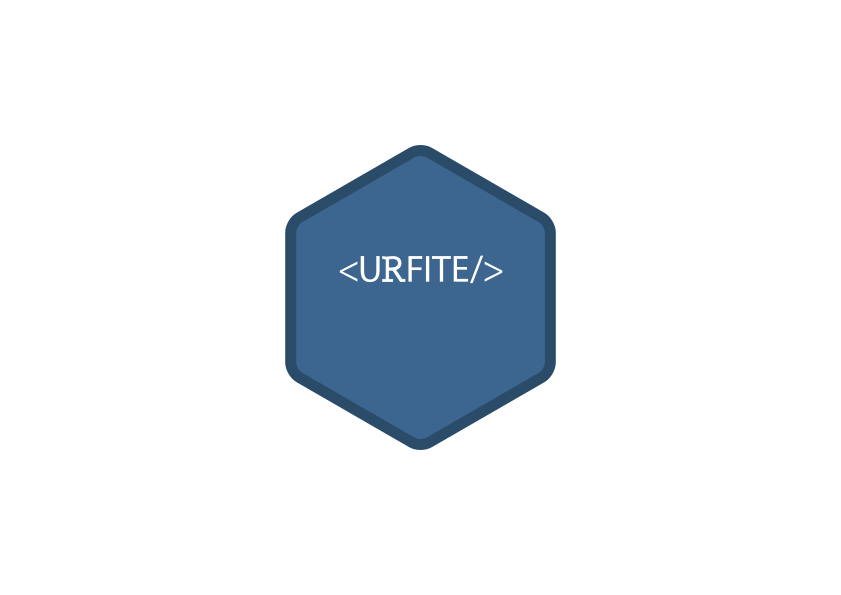
\includegraphics[width=0.45\linewidth]{images/URFITE_logo} \end{center}

\noindent\rule{\textwidth}{1pt}

The interest in the freely available statistical programming language
and software environment \texttt{R} \citep{R-base} is soaring. By the
time we wrote first drafts for this project, more than 11000 addons
(many of them providing cutting-edge methods) were made available on the
Comprehensive \texttt{R} Archive Network
(\href{https://cran.r-project.org/}{CRAN}), an extensive network of FTP
servers around the world that store identical and up-to-date versions of
\texttt{R} code and its documentation. \texttt{R} dominates other
(commercial) software for statistical computing in most fields of
research in applied statistics. The benefits of it being freely
available, open source and having a large and constantly growing
community of users that contribute to CRAN render \texttt{R} more and
more appealing for empirical economists and econometricians alike.

A striking advantage of using \texttt{R} in econometrics is that it
enables students to explicitly document their analysis step-by-step such
that it is easy to update and to expand. This allows to re-use code for
similar applications with different data. Furthermore, \texttt{R}
programs are fully reproducible, which makes it straightforward for
others to comprehend and validate results.

Over the recent years, \texttt{R} has thus become an integral part of
the curricula of econometrics classes we teach at the University of
Duisburg-Essen. In some sense, learning to code is comparable to
learning a foreign language and continuous practice is essential for the
learning success. Needless to say, presenting bare \texttt{R} code on
slides does not encourage the students to engage with hands-on
experience on their own. This is why \texttt{R} is crucial. As for
accompanying literature, there are some excellent books that deal with
\texttt{R} and its applications to econometrics
\citep[e.g.][]{kleiber2008}. However, such sources beyond the scope of
undergraduate students in economics having little understanding of
econometric methods and barely any experience in programming at all.
Consequently, we started to compile a collection of reproducible reports
for use in class. These reports provide guidance on how to implement
selected applications from the textbook \emph{Introduction to
Econometrics} \citep{stock2015} which serves as a basis for the lecture
and the accompanying tutorials. The process is facilitated considerably
by \texttt{knitr} \citep{R-knitr} and \texttt{rmarkdown}
\citep{R-rmarkdown}. In conjunction, both \texttt{R} packages provide
powerful tools for dynamic report generation which allow to seamlessly
combine pure text, LaTeX, \texttt{R} code and its output in a variety of
formats, including PDF and HTML. Being inspired by \emph{Using R for
Introductory Econometrics} \citep{heiss2016}\footnote{\citet{heiss2016}
  builds on the popular \emph{Introductory Econometrics} by
  \citet{wooldridge2016} and demonstrates how to replicate the
  applications discussed therein using \texttt{R}.} and with this
powerful toolkit at hand we wrote up our own empirical companion to
\citet{stock2015}, the result which you to look at, is \textbf{U}sing
\textbf{R} \textbf{f}or \textbf{I}ntroduction \textbf{t}o
\textbf{E}conometrics (\emph{URFITE}).

Similarly to the book by \citet{heiss2016} this project is neither a
comprehensive econometrics textbook nor is it intended to be a general
introduction \texttt{R}. We feel that Stock and Watson do a great job at
explaining the intuition and theory of econometrics, and at any rate
better than we could in yet another introductory textbook! \emph{URFITE}
is best described as an interactive script in the style of a
reproducible research report which aims to provide students with a
platform-independent e-learning arrangement by seamlessly intertwining
theoretical core knowledge and empirical skills in undergraduate
econometrics. Of course, the focus is on empirical applications with
\texttt{R}. We leave out derivations and proofs wherever we can. Our
goal is to enable students not only to learn how results of case studies
can be replicated with \texttt{R} but we also intend to strengthen their
ability in using the newly acquired skills in other empirical
applications --- immediately within \emph{URFITE}.

To realize this, each chapter contains interactive \texttt{R}
programming exercises. These exercises are used as supplements to code
chunks that display how previously discussed techniques can be
implemented within \texttt{R}. They are generated using the
\href{https://github.com/datacamp/datacamp-light}{DataCamp light widget}
and are backed by an \texttt{R} session which is maintained on
\href{https://www.datacamp.com/home}{DataCamp}'s servers. You may play
around with the example exercise presented below.

\begin{center}\textit{This interactive application is only available in the HTML version.}\end{center}

As you can see above, the widget consists of two tabs. \texttt{script.R}
mimics an \texttt{.R}-file, a file format that is commonly used for
storing \texttt{R} code. Lines starting with a \# are commented out,
that is, they are not recognized as code. Furthermore, \texttt{script.R}
works like an exercise sheet where you may write down the solution you
come up with. If you hit the button \emph{Run}, the code will be
executed, submission correctness tests are run and you will be notified
whether your approach is correct. If it is not correct, you will receive
feedback suggesting improvements or hints. The other tab,
\texttt{R Console}, is a fully functional \texttt{R} console that can be
used for trying out solutions to exercises before submitting them. Of
course you may submit (almost any) \texttt{R} code and use the console
to play around and explore. Simply type a command and hit the enter key
on your keyboard.

As an example, consider the following line of code presented in chunk
below. It tells \texttt{R} to compute the number of packages available
on \texttt{CRAN}. The code chunk is followed by the output produced.

\begin{Shaded}
\begin{Highlighting}[]
\CommentTok{# compute the number of packages available on CRAN}
\KeywordTok{nrow}\NormalTok{(}\KeywordTok{available.packages}\NormalTok{(}\DataTypeTok{repos =} \StringTok{"http://cran.us.r-project.org"}\NormalTok{))}
\end{Highlighting}
\end{Shaded}

\begin{verbatim}
## [1] 12773
\end{verbatim}

Each code chunk is equipped with a button on the outer right hand side
which copies the code to your clipboard. This makes it convenient to
work with larger code segments. In the widget above, you may click on
\texttt{R Console} and type \texttt{nrow(available.packages())} (the
command from the code chunk above) and execute it by hitting
\emph{Enter} on your keyboard\footnote{The \texttt{R} session is
  initialized by clicking anywhere into the widget. This might take a
  few seconds. Just wait for the indicator next to the button \emph{Run}
  to turn green.}

Note that some lines in the widget are out-commented which ask you to
assign a numeric value to a variable and then to print the variable's
content to the console. You may enter your solution approach to
\texttt{script.R} and hit the button \emph{Run} in order to get the
feedback described further above. In case you do not know how to solve
this sample exercise (don't panic, that is probably why you are reading
this), a click on \emph{Hint} will provide you with some advice. If you
still can't find a solution, a click on \emph{Solution} will provide you
with another tab, \texttt{Solution.R} which contains sample solution
code. It will often be the case that exercises can be solved in many
different ways and \texttt{Solution.R} presents what we consider as
comprehensible and idiomatic.

\subsubsection*{Conventions Used in this
Book}\label{conventions-used-in-this-book}
\addcontentsline{toc}{subsubsection}{Conventions Used in this Book}

\begin{itemize}
\item
  \emph{Italic} text indicates new terms, names, buttons and alike.
\item
  \texttt{Constant width text}, is generally used in paragraphs to refer
  to \texttt{R} code. This includes commands, variables, functions, data
  types, databases and file names.
\item
  Constant width text on gray background is used to indicate \texttt{R}
  code that can be typed literally by you. It may appear in paragraphs
  for better distinguishability among executable and non-executable code
  statements but it will mostly be encountered in shape of large blocks
  of \texttt{R} code. These blocks are referred to as code chunks (see
  above).
\end{itemize}

\subsubsection*{Acknowledgements}\label{acknowledgements}
\addcontentsline{toc}{subsubsection}{Acknowledgements}

We thank Alexander Blasberg and Kim Hermann for proofreading and their
constructive criticism. We also thank the \emph{Stiferverband für die
Deutsche Wissenschaft e.V.} and the Ministry of Science and Research
North Rhine-Westphalia for their financial support. We are also indebted
to all past students of our introductory econometrics courses at the
University of Duisburg-Essen for their feedback.

\section{\texorpdfstring{A Very Short Introduction to \texttt{R} and
\emph{RStudio}}{A Very Short Introduction to  and RStudio}}\label{a-very-short-introduction-to-and-rstudio}

\begin{figure}[h]

{\centering \includegraphics[width=1\linewidth]{images/rstudio} 

}

\caption{RStudio: the four panes}\label{fig:unnamed-chunk-7}
\end{figure}

\subsubsection*{\texorpdfstring{\texttt{R}
Basics}{ Basics}}\label{basics}
\addcontentsline{toc}{subsubsection}{\texttt{R} Basics}

As mentioned before, this book is not intended to be an introduction to
\texttt{R} but as a guide on how to use its capabilities for
applications commonly encountered in undergraduate econometrics. Those
having basic knowledge in \texttt{R} programming will feel comfortable
starting with Chapter \ref{pt}. This section, however, is meant for
those who have not worked with \texttt{R} or \emph{RStudio} before. If
you at least know how to create objects and call functions, you can skip
it. If you would like to refresh your skills or get a feeling for how to
work with \emph{RStudio}, keep reading.

First of all start \emph{RStudio} and create a new \texttt{R} script by
selecting \emph{File}, \emph{New File}, \emph{R Script}. In the editor
pane, type

\begin{Shaded}
\begin{Highlighting}[]
\DecValTok{1} \OperatorTok{+}\StringTok{ }\DecValTok{1}
\end{Highlighting}
\end{Shaded}

and click on the button labeled \emph{Run} in the top right corner of
the editor. By doing so, your line of code is sent to the console and
the result of this operation should be displayed right underneath it. As
you can see, \texttt{R} works just like a calculator. You can do all
arithmetic calculations by using the corresponding operator (\texttt{+},
\texttt{-}, \texttt{*}, \texttt{/} or \texttt{\textasciicircum{}}). If
you are not sure what the last operator does, try it out and check the
results.

\subsubsection*{Vectors}\label{vectors}
\addcontentsline{toc}{subsubsection}{Vectors}

\texttt{R} is of course more sophisticated than that. We can work with
variables or, more generally, objects. Objects are defined by using the
assignment operator \texttt{<-}. To create a variable named \texttt{x}
which contains the value \texttt{10} type \texttt{x\ \textless{}-\ 10}
and click the button \emph{Run} yet again. The new variable should have
appeared in the environment pane on the top right. The console however
did not show any results, because our line of code did not contain any
call that creates output. When you now type \texttt{x} in the console
and hit return, you ask \texttt{R} to show you the value of \texttt{x}
and the corresponding value should be printed in the console.

\texttt{x} is a scalar, a vector of length \(1\). You can easily create
longer vectors by using the function \texttt{c()} (\emph{c} for
``concatenate'' or ``combine''). To create a vector \texttt{y}
containing the numbers \(1\) to \(5\) and print it, do the following.

\begin{Shaded}
\begin{Highlighting}[]
\NormalTok{y <-}\StringTok{ }\KeywordTok{c}\NormalTok{(}\DecValTok{1}\NormalTok{, }\DecValTok{2}\NormalTok{, }\DecValTok{3}\NormalTok{, }\DecValTok{4}\NormalTok{, }\DecValTok{5}\NormalTok{)}
\NormalTok{y}
\end{Highlighting}
\end{Shaded}

\begin{verbatim}
## [1] 1 2 3 4 5
\end{verbatim}

You can also create a vector of letters or words. For now just remember
that characters have to be surrounded by quotes, else they will be
parsed as object names.

\begin{Shaded}
\begin{Highlighting}[]
\NormalTok{hello <-}\StringTok{ }\KeywordTok{c}\NormalTok{(}\StringTok{"Hello"}\NormalTok{, }\StringTok{"World"}\NormalTok{)}
\end{Highlighting}
\end{Shaded}

Here we have created a vector of length 2 containing the words
\texttt{Hello} and \texttt{World}.

Do not forget to save your script! To do so, select \emph{File},
\emph{Save}.

\subsubsection*{Functions}\label{functions}
\addcontentsline{toc}{subsubsection}{Functions}

You have seen the function \texttt{c()} that can be used to combine
objects. In general, all function calls look the same: a function name
is always followed by round parentheses. Sometimes, the parentheses
include arguments.

Here are two simple examples.

\begin{Shaded}
\begin{Highlighting}[]
\NormalTok{z <-}\StringTok{ }\KeywordTok{seq}\NormalTok{(}\DataTypeTok{from =} \DecValTok{1}\NormalTok{, }\DataTypeTok{to =} \DecValTok{5}\NormalTok{, }\DataTypeTok{by =} \DecValTok{1}\NormalTok{)}

\KeywordTok{mean}\NormalTok{(}\DataTypeTok{x =}\NormalTok{ z)}
\end{Highlighting}
\end{Shaded}

\begin{verbatim}
## [1] 3
\end{verbatim}

In the first line we use a function called \texttt{seq()} to create the
exact same vector as we did in the previous section, calling it
\texttt{z}. The function takes on the arguments \texttt{from},
\texttt{to} and \texttt{by} which should be self-explanatory. The
function \texttt{mean()} computes the arithmetic mean of its argument
\texttt{x}. Since we pass the vector \texttt{z} as the argument
\texttt{x}, the result is \texttt{3}!

If you are not sure which arguments a function expects, you may consult
the function's documentation. Let's say we are not sure how the
arguments required for \texttt{seq()} work. We then type \texttt{?seq}
in the console. By hitting return the documentation page for that
function pops up in the lower right pane of \emph{RStudio}. In there,
the section \emph{Arguments} holds the information we seek. On the
bottom of almost every help page you find examples on how to use the
corresponding functions. This is very helpful for beginners and we
recommend to look out for those.

Of course, all of the commands presented above also work in interactive
widgets throughout the book. You may try them below.

\begin{center}\textit{This interactive application is only available in the HTML version.}\end{center}

\chapter{Linear Regression with One Regressor}\label{lrwor}

This chapter introduces the basics in linear regression and shows how to
perform regression analysis in \texttt{R}. In linear regression, the aim
is to model the relationship between a dependent variable \(Y\) and one
or more explanatory variables denoted by \(X_1, X_2, \dots, X_k\).
Following the book we will focus on the concept of simple linear
regression throughout the whole chapter. In simple linear regression,
there is just one explanatory variable \(X_1\). If, for example, a
school cuts its class sizes by hiring new teachers, that is, the school
lowers \(X_1\), the student-teacher ratios of its classes, how would
this affect \(Y\), the performance of the students involved in a
standardized test? With linear regression we can not only examine
whether the student-teacher ratio \emph{does have} an impact on the test
results but we can also learn about the \emph{direction} and the
\emph{strength} of this effect.

The following packages are needed for reproducing the code presented in
this chapter:

\begin{itemize}
\item
  \texttt{AER} - accompanies the Book \emph{Applied Econometrics with R}
  \citet{kleiber2008} and provides useful functions and data sets.
\item
  \texttt{MASS} - a collection of functions for applied statistics.
\end{itemize}

Make sure these are installed before you go ahead and try to replicate
the examples. The safest way to do so is by checking whether the
following code chunk executes without any errors.

\begin{Shaded}
\begin{Highlighting}[]
\KeywordTok{library}\NormalTok{(AER)}
\KeywordTok{library}\NormalTok{(MASS)}
\end{Highlighting}
\end{Shaded}

\section{Simple Linear Regression}\label{simple-linear-regression}

To start with an easy example, consider the following combinations of
average test score and the average student-teacher ratio in some
fictional school districts.

\begin{table}[H]
\centering
\begin{tabular}{lrrrrrrr}
\toprule
  & 1 & 2 & 3 & 4 & 5 & 6 & 7\\
\midrule
TestScore & 680 & 640 & 670 & 660 & 630 & 660.0 & 635\\
STR & 15 & 17 & 19 & 20 & 22 & 23.5 & 25\\
\bottomrule
\end{tabular}
\end{table}

To work with these data in \texttt{R} we begin by generating two
vectors: one for the student-teacher ratios (\texttt{STR}) and one for
test scores (\texttt{TestScore}), both containing the data from the
table above.

\begin{Shaded}
\begin{Highlighting}[]
\CommentTok{# Create sample data}
\NormalTok{STR <-}\StringTok{ }\KeywordTok{c}\NormalTok{(}\DecValTok{15}\NormalTok{, }\DecValTok{17}\NormalTok{, }\DecValTok{19}\NormalTok{, }\DecValTok{20}\NormalTok{, }\DecValTok{22}\NormalTok{, }\FloatTok{23.5}\NormalTok{, }\DecValTok{25}\NormalTok{)}
\NormalTok{TestScore <-}\StringTok{ }\KeywordTok{c}\NormalTok{(}\DecValTok{680}\NormalTok{, }\DecValTok{640}\NormalTok{, }\DecValTok{670}\NormalTok{, }\DecValTok{660}\NormalTok{, }\DecValTok{630}\NormalTok{, }\DecValTok{660}\NormalTok{, }\DecValTok{635}\NormalTok{) }

\CommentTok{# Print out sample data}
\NormalTok{STR}
\end{Highlighting}
\end{Shaded}

\begin{verbatim}
## [1] 15.0 17.0 19.0 20.0 22.0 23.5 25.0
\end{verbatim}

\begin{Shaded}
\begin{Highlighting}[]
\NormalTok{TestScore}
\end{Highlighting}
\end{Shaded}

\begin{verbatim}
## [1] 680 640 670 660 630 660 635
\end{verbatim}

In a simple linear regression model, we model the relationship between
both variables by a straight line, formally \[ Y = b \cdot X + a. \] For
now, let us suppose that the function which relates test score and
student-teacher ratio to each other is
\[TestScore = 713 - 3 \times STR.\]

It is always a good idea to visualize the data you work with. Here, it
is suitable to use \texttt{plot()} to produce a scatterplot with
\texttt{STR} on the \(x\)-axis and \texttt{TestScore} on the \(y\)-axis.
Just call \texttt{plot(y\_variable\ \textasciitilde{}\ x\_variable)}
whereby \texttt{y\_variable} and \texttt{x\_variable} are placeholders
for the vectors of observations we want to plot. Furthermore, we might
want to add a systematic relationship to the plot. To draw a straight
line, \texttt{R} provides the function \texttt{abline()}. We just have
to call this function with arguments \texttt{a} (representing the
intercept) and \texttt{b} (representing the slope) after executing
\texttt{plot()} in order to add the line to our plot.

The following code reproduces Figure 4.1 from the textbook.

\begin{Shaded}
\begin{Highlighting}[]
\CommentTok{# create a scatterplot of the data}
\KeywordTok{plot}\NormalTok{(TestScore }\OperatorTok{~}\StringTok{ }\NormalTok{STR)}

\CommentTok{# add the systematic relationship to the plot}
\KeywordTok{abline}\NormalTok{(}\DataTypeTok{a =} \DecValTok{713}\NormalTok{, }\DataTypeTok{b =} \OperatorTok{-}\DecValTok{3}\NormalTok{)}
\end{Highlighting}
\end{Shaded}

\begin{center}\includegraphics{URFITE_files/figure-latex/unnamed-chunk-16-1} \end{center}

We find that the line does not touch any of the points although we
claimed that it represents the systematic relationship. The reason for
this is randomness. Most of the time there are additional influences
which imply that there is no bivariate relationship between the two
variables.

In order to account for these differences between observed data and the
systematic relationship, we extend our model from above by an
\emph{error term} \(u\) which captures additional random effects. Put
differently, \(u\) accounts for all the differences between the
regression line and the actual observed data. Beside pure randomness,
these deviations could also arise from measurement errors or, as will be
discussed later, could be the consequence of leaving out other factors
that are relevant in explaining the dependent variable.

Which other factors are plausible in our example? For one thing, the
test scores might be driven by the teachers' quality and the background
of the students. It is also possible that in some classes, the students
were lucky on the test days and thus achieved higher scores. For now, we
will summarize such influences by an additive component:

\[ TestScore = \beta_0 + \beta_1 \times STR + \text{other factors} \]

Of course this idea is very general as it can be easily extended to
other situations that can be described with a linear model. The basic
linear regression function we will work with hence is

\[ Y_i = \beta_0 + \beta_1 X_i + u_i. \]

Key Concept 4.1 summarizes the terminology of the simple linear
regression model.

\begin{keyconcepts}[Terminology for the Linear Regression Model with a Single Regressor]{4.1}
The linear regression model is $$Y_i = \beta_0 + \beta_1 X_1 + u_i$$
where
\begin{itemize}
\item the index $i$ runs over the observations, $i=1,\dots,n$
\item $Y_i$ is the \textit{dependent variable}, the \textit{regressand}, or simply the \textit{left-hand variable}
\item $X_i$ is the \textit{independent variable}, the \textit{regressor}, or simply the \textit{right-hand variable}
\item $Y = \beta_0 + \beta_1 X$ is the \textit{population regression line} also called the \textit{population regression function}
\item $\beta_0$ is the \textit{intercept} of the population regression line
\item $\beta_1$ is the \textit{slope} of the population regression line
\item $u_i$ is the \textit{error term}.
\end{itemize}
\end{keyconcepts}

\section{Estimating the Coefficients of the Linear Regression
Model}\label{estimating-the-coefficients-of-the-linear-regression-model}

In practice, the intercept \(\beta_0\) and slope \(\beta_1\) of the
population regression line are unknown. Therefore, we must employ data
to estimate both unknown parameters. In the following, a real world
example will be used to demonstrate how this is achieved. We want to
relate test scores to student-teacher ratios measured in Californian
schools. The test score is the district-wide average of reading and math
scores for fifth graders. Again, the class size is measured as the
number of students divided by the number of teachers (the
student-teacher ratio). As for the data, the California School data set
(\texttt{CASchools}) comes with an \texttt{R} package called
\texttt{AER}, an acronym for
\href{https://cran.r-project.org/web/packages/AER/AER.pdf}{Applied
Econometrics with R} \citep{R-AER}. After installing the package with
\texttt{install.packages("AER")} and attaching it with
\texttt{library(AER)} the data set can be loaded using the function
\texttt{data()}.

\begin{Shaded}
\begin{Highlighting}[]
\CommentTok{# install the AER package (once)}
\KeywordTok{install.packages}\NormalTok{(}\StringTok{"AER"}\NormalTok{)}

\CommentTok{# load the AER package }
\KeywordTok{library}\NormalTok{(AER)   }

\CommentTok{# load the the data set in the workspace}
\KeywordTok{data}\NormalTok{(CASchools) }
\end{Highlighting}
\end{Shaded}

Once a package has been installed it is available for use at further
occasions when invoked with \texttt{library()} --- there is no need to
run \texttt{install.packages()} again!

It is interesting to know what kind of object we are dealing with.
\texttt{class()} returns the class of an object. Depending on the class
of an object some functions (for example \texttt{plot()} and
\texttt{summary()}) behave differently.

Let us check the class of the object \texttt{CASchools}.

\begin{Shaded}
\begin{Highlighting}[]
\KeywordTok{class}\NormalTok{(CASchools)}
\end{Highlighting}
\end{Shaded}

\begin{verbatim}
## [1] "data.frame"
\end{verbatim}

It turns out that \texttt{CASchools} is of class \texttt{data.frame}
which is a convenient format to work with, especially for performing
regression analysis.

With help of \texttt{head()} we get a first overview of our data. This
function shows only the first 6 rows of the data set which prevents an
overcrowded console output.

\BeginKnitrBlock{rmdnote}
Press ctrl + L to clear the console. This command deletes any code that
has been typed in and executed by you or printed to the console by R
functions. The good news is that anything else is left untouched. You
neither loose defined variables etc. nor the code history. It is still
possible to recall previously executed R commands using the up and down
keys. If you are working in \emph{RStudio}, press ctrl + Up on your
keyboard (CMD + Up on a Mac) to review a list of previously entered
commands.
\EndKnitrBlock{rmdnote}

\begin{Shaded}
\begin{Highlighting}[]
\KeywordTok{head}\NormalTok{(CASchools)}
\end{Highlighting}
\end{Shaded}

\begin{verbatim}
##   district                          school  county grades students
## 1    75119              Sunol Glen Unified Alameda  KK-08      195
## 2    61499            Manzanita Elementary   Butte  KK-08      240
## 3    61549     Thermalito Union Elementary   Butte  KK-08     1550
## 4    61457 Golden Feather Union Elementary   Butte  KK-08      243
## 5    61523        Palermo Union Elementary   Butte  KK-08     1335
## 6    62042         Burrel Union Elementary  Fresno  KK-08      137
##   teachers calworks   lunch computer expenditure    income   english  read
## 1    10.90   0.5102  2.0408       67    6384.911 22.690001  0.000000 691.6
## 2    11.15  15.4167 47.9167      101    5099.381  9.824000  4.583333 660.5
## 3    82.90  55.0323 76.3226      169    5501.955  8.978000 30.000002 636.3
## 4    14.00  36.4754 77.0492       85    7101.831  8.978000  0.000000 651.9
## 5    71.50  33.1086 78.4270      171    5235.988  9.080333 13.857677 641.8
## 6     6.40  12.3188 86.9565       25    5580.147 10.415000 12.408759 605.7
##    math
## 1 690.0
## 2 661.9
## 3 650.9
## 4 643.5
## 5 639.9
## 6 605.4
\end{verbatim}

We find that the data set consists of plenty of variables and that most
of them are numeric.

By the way: an alternative to \texttt{class()} and \texttt{head()} is
\texttt{str()} which is deduced from `structure' and gives a
comprehensive overview of the object. Try!

Turning back to \texttt{CASchools}, the two variables we are interested
in (i.e., average test score and the student-teacher ratio) are
\emph{not} included. However, it is possible to calculate both from the
provided data. To obtain the student-teacher ratios, we simply divide
the number of students by the number of teachers. The average test score
is the arithmetic mean of the test score for reading and the score of
the math test. The next code chunk shows how the two variables can be
constructed as vectors and how they are appended to \texttt{CASchools}.

\begin{Shaded}
\begin{Highlighting}[]
\CommentTok{# compute STR and append it to CASchools}
\NormalTok{CASchools}\OperatorTok{$}\NormalTok{STR <-}\StringTok{ }\NormalTok{CASchools}\OperatorTok{$}\NormalTok{students}\OperatorTok{/}\NormalTok{CASchools}\OperatorTok{$}\NormalTok{teachers }

\CommentTok{# compute TestScore and append it to CASchools}
\NormalTok{CASchools}\OperatorTok{$}\NormalTok{score <-}\StringTok{ }\NormalTok{(CASchools}\OperatorTok{$}\NormalTok{read }\OperatorTok{+}\StringTok{ }\NormalTok{CASchools}\OperatorTok{$}\NormalTok{math)}\OperatorTok{/}\DecValTok{2}     
\end{Highlighting}
\end{Shaded}

If we ran \texttt{head(CASchools)} again we would find the two variables
of interest as additional columns named \texttt{STR} and \texttt{score}
(check this!).

Table 4.1 from the textbook summarizes the distribution of test scores
and student-teacher ratios. There are several functions which can be
used to produce similar results, e.g.,

\begin{itemize}
\item
  \texttt{mean()} (computes the arithmetic mean of the provided numbers)
\item
  \texttt{sd()} (computes the sample standard deviation)
\item
  \texttt{quantile()} (returns a vector of the specified sample
  quantiles for the data).
\end{itemize}

The next code chunk shows how to achieve this. First, we compute summary
statistics on the columns \texttt{STR} and \texttt{score} of
\texttt{CASchools}. In order to get nice output we gather the measures
in a \texttt{data.frame} named \texttt{DistributionSummary}.

\begin{Shaded}
\begin{Highlighting}[]
\CommentTok{# compute sample averages of STR and score}
\NormalTok{avg_STR <-}\StringTok{ }\KeywordTok{mean}\NormalTok{(CASchools}\OperatorTok{$}\NormalTok{STR) }
\NormalTok{avg_score <-}\StringTok{ }\KeywordTok{mean}\NormalTok{(CASchools}\OperatorTok{$}\NormalTok{score)}

\CommentTok{# compute sample standard deviations of STR and score}
\NormalTok{sd_STR <-}\StringTok{ }\KeywordTok{sd}\NormalTok{(CASchools}\OperatorTok{$}\NormalTok{STR) }
\NormalTok{sd_score <-}\StringTok{ }\KeywordTok{sd}\NormalTok{(CASchools}\OperatorTok{$}\NormalTok{score)}

\CommentTok{# set up a vector of percentiles and compute the quantiles }
\NormalTok{quantiles <-}\StringTok{ }\KeywordTok{c}\NormalTok{(}\FloatTok{0.10}\NormalTok{, }\FloatTok{0.25}\NormalTok{, }\FloatTok{0.4}\NormalTok{, }\FloatTok{0.5}\NormalTok{, }\FloatTok{0.6}\NormalTok{, }\FloatTok{0.75}\NormalTok{, }\FloatTok{0.9}\NormalTok{)}
\NormalTok{quant_STR <-}\StringTok{ }\KeywordTok{quantile}\NormalTok{(CASchools}\OperatorTok{$}\NormalTok{STR, quantiles)}
\NormalTok{quant_score <-}\StringTok{ }\KeywordTok{quantile}\NormalTok{(CASchools}\OperatorTok{$}\NormalTok{score, quantiles)}

\CommentTok{# gather everything in a data.frame }
\NormalTok{DistributionSummary <-}\StringTok{ }\KeywordTok{data.frame}\NormalTok{(}
                                  \DataTypeTok{Average =} \KeywordTok{c}\NormalTok{(avg_STR, avg_score), }
                                  \DataTypeTok{StandardDeviation =} \KeywordTok{c}\NormalTok{(sd_STR, sd_score), }
                                  \DataTypeTok{quantile =} \KeywordTok{rbind}\NormalTok{(quant_STR, quant_score)}
\NormalTok{                                  )}

\CommentTok{# print the summary to the console}
\NormalTok{DistributionSummary}
\end{Highlighting}
\end{Shaded}

\begin{verbatim}
##               Average StandardDeviation quantile.10. quantile.25.
## quant_STR    19.64043          1.891812      17.3486     18.58236
## quant_score 654.15655         19.053347     630.3950    640.05000
##             quantile.40. quantile.50. quantile.60. quantile.75.
## quant_STR       19.26618     19.72321      20.0783     20.87181
## quant_score    649.06999    654.45000     659.4000    666.66249
##             quantile.90.
## quant_STR       21.86741
## quant_score    678.85999
\end{verbatim}

As for the sample data, we use \texttt{plot()}. This allows us to detect
characteristics of our data, such as outliers which are harder to
discover by looking at mere numbers. This time we add some additional
arguments to the call of \texttt{plot()}.

The first argument in our call of \texttt{plot()},
\texttt{score \textasciitilde{} STR}, is again a formula that variables.
However, this time the two variables are not saved in separate vectors
but are columns of \texttt{CASchools}. Therefore, \texttt{R} would not
find them without the argument \texttt{data} being correctly specified.
\texttt{data} must be in accordance with the name of the
\texttt{data.frame} to which the variables belong to, in this case
\texttt{CASchools}. Further arguments are used to change the appearance
of the plot: while \texttt{main} adds a title, \texttt{xlab} and
\texttt{ylab} add custom labels to both axes.

\begin{Shaded}
\begin{Highlighting}[]
\KeywordTok{plot}\NormalTok{(score }\OperatorTok{~}\StringTok{ }\NormalTok{STR, }
     \DataTypeTok{data =}\NormalTok{ CASchools,}
     \DataTypeTok{main =} \StringTok{"Scatterplot of TestScore and STR"}\NormalTok{, }
     \DataTypeTok{xlab =} \StringTok{"STR (X)"}\NormalTok{,}
     \DataTypeTok{ylab =} \StringTok{"Test Score (Y)"}\NormalTok{)}
\end{Highlighting}
\end{Shaded}

\begin{center}\includegraphics{URFITE_files/figure-latex/unnamed-chunk-24-1} \end{center}

The plot (Figure 4.2 in the book) shows the scatterplot of all
observations on the student-teacher ratio and test score. We see that
the points are strongly scattered, and that the variables are negatively
correlated. That is, we expect to observe lower test scores in bigger
classes.

The function \texttt{cor()} (see \texttt{?cor} for further info) can be
used to compute the correlation between two \emph{numeric} vectors.

\begin{Shaded}
\begin{Highlighting}[]
\KeywordTok{cor}\NormalTok{(CASchools}\OperatorTok{$}\NormalTok{STR, CASchools}\OperatorTok{$}\NormalTok{score)}
\end{Highlighting}
\end{Shaded}

\begin{verbatim}
## [1] -0.2263627
\end{verbatim}

As the scatterplot already suggests, the correlation is negative but
rather weak.

The task we are now faceing is to find a line which best fits the data.
Of course we could simply stick with graphical inspection and
correlation analysis and then select the best fitting line by
eyeballing. However, this would be rather subjective: different
observers would draw different regression lines. On this account, we are
interested in techniques that are less arbitrary. Such a technique is
given by ordinary least squares (OLS) estimation.

\subsection*{The Ordinary Least Squares
Estimator}\label{the-ordinary-least-squares-estimator}
\addcontentsline{toc}{subsection}{The Ordinary Least Squares Estimator}

The OLS estimator chooses the regression coefficients such that the
estimated regression line is as ``close'' as possible to the observed
data points. Here, closeness is measured by the sum of the squared
mistakes made in predicting \(Y\) given \(X\). Let \(b_0\) and \(b_1\)
be some estimators of \(\beta_0\) and \(\beta_1\). Then the sum of
squared estimation mistakes can be expressed as

\[ \sum^n_{i = 1} (Y_i - b_0 - b_1 X_i)^2. \]

The OLS estimator in the simple regression model is the pair of
estimators for intercept and slope which minimizes the expression above.
The derivation of the OLS estimators for both parameters are presented
in Appendix 4.1 of the book. The results are summarized in Key Concept
4.2.

\begin{keyconcepts}[The OLS Estimator, Predicted Values, and Residuals]{4.2}
The OLS estimators of the slope $\beta_1$ and the intercept $\beta_0$ in the simple linear regression model are
\begin{align*}
  \hat\beta_1 & = \frac{ \sum_{i = 1}^n (X_i - \overline{X})(Y_i - \overline{Y}) } { \sum_{i=1}^n (X_i - \overline{X})^2},  \\
\hat\beta_0 & =  \overline{Y} - \hat\beta_1 \overline{X}. 
\intertext{The OLS predicted values $\widehat{Y}_i$ and residuals $\hat{u}_i$ are}
  \widehat{Y}_i & =  \hat\beta_0 + \hat\beta_1 X_i,\\
  \hat{u}_i & =  Y_i - \widehat{Y}_i. 
\end{align*}

The estimated intercept $\hat{\beta}_0$, the slope parameter $\hat{\beta}_1$ and the residuals $\left(\hat{u}_i\right)$ are computed from a sample of $n$ observations of $X_i$ and $Y_i$, $i$, $...$,  $n$. These are \textit{estimates} of the unknown true population intercept $\left(\beta_0 \right)$, slope $\left(\beta_1\right)$, and error term $(u_i)$.
\end{keyconcepts}

The formulas presented above may not be very intuitive at first glance.
The following interactive application aims to help you understand the
mechanics of OLS. You can add observations by clicking into the
coordinate system where the data are represented by points. Once two or
more observations are available, the application computes a regression
line using OLS and some statistics which are displayed in the right
panel. The results are updated as you add further observations to the
left panel. A double-click resets the application, i.e., all data are
removed.

There are many possible ways to compute \(\hat{\beta}_0\) and
\(\hat{\beta}_1\) in \texttt{R}. For example, we could implement the
formulas presented in Key Concept 4.2 with two of \texttt{R}'s most
basic functions: \texttt{mean()} and \texttt{sum()}.

\begin{Shaded}
\begin{Highlighting}[]
\KeywordTok{attach}\NormalTok{(CASchools) }\CommentTok{# allows to use the variables contained in CASchools directly}

\CommentTok{# compute beta_1_hat}
\NormalTok{beta_}\DecValTok{1}\NormalTok{ <-}\StringTok{ }\KeywordTok{sum}\NormalTok{((STR }\OperatorTok{-}\StringTok{ }\KeywordTok{mean}\NormalTok{(STR))}\OperatorTok{*}\NormalTok{(score }\OperatorTok{-}\StringTok{ }\KeywordTok{mean}\NormalTok{(score))) }\OperatorTok{/}\StringTok{ }\KeywordTok{sum}\NormalTok{((STR }\OperatorTok{-}\StringTok{ }\KeywordTok{mean}\NormalTok{(STR))}\OperatorTok{^}\DecValTok{2}\NormalTok{)}

\CommentTok{# compute beta_0_hat}
\NormalTok{beta_}\DecValTok{0}\NormalTok{ <-}\StringTok{ }\KeywordTok{mean}\NormalTok{(score) }\OperatorTok{-}\StringTok{ }\NormalTok{beta_}\DecValTok{1} \OperatorTok{*}\StringTok{ }\KeywordTok{mean}\NormalTok{(STR)}

\CommentTok{# print the results to the console}
\NormalTok{beta_}\DecValTok{1}
\end{Highlighting}
\end{Shaded}

\begin{verbatim}
## [1] -2.279808
\end{verbatim}

\begin{Shaded}
\begin{Highlighting}[]
\NormalTok{beta_}\DecValTok{0}
\end{Highlighting}
\end{Shaded}

\begin{verbatim}
## [1] 698.9329
\end{verbatim}

Of course, there are even more manual ways to perform these tasks. With
OLS being one of the most widely-used estimation techniques, \texttt{R}
of course already contains a built-in function named \texttt{lm()}
(\textbf{l}inear \textbf{m}odel) which can be used to carry out
regression analysis.

The first argument of the function to be specified is, similar to
\texttt{plot()}, the regression formula with the basic syntax
\texttt{y \textasciitilde{} x} where \texttt{y} is the dependent
variable and \texttt{x} the explanatory variable. The argument
\texttt{data} determines the data set to be used in the regression. We
now revisit the example from the book where the relationship between the
test scores and the class sizes is analyzed. The following code uses
\texttt{lm()} to replicate the results presented in figure 4.3 of the
book.

\begin{Shaded}
\begin{Highlighting}[]
\CommentTok{# estimate the model and assign the result to linear_model}
\NormalTok{linear_model <-}\StringTok{ }\KeywordTok{lm}\NormalTok{(score }\OperatorTok{~}\StringTok{ }\NormalTok{STR, }\DataTypeTok{data =}\NormalTok{ CASchools)}

\CommentTok{# print the standard output of the estimated lm object to the console }
\NormalTok{linear_model}
\end{Highlighting}
\end{Shaded}

\begin{verbatim}
## 
## Call:
## lm(formula = score ~ STR, data = CASchools)
## 
## Coefficients:
## (Intercept)          STR  
##      698.93        -2.28
\end{verbatim}

Let us add the estimated regression line to the plot. This time we also
enlarge the ranges of both axes by setting the arguments \texttt{xlim}
and \texttt{ylim}.

\begin{Shaded}
\begin{Highlighting}[]
\CommentTok{# plot the data}
\KeywordTok{plot}\NormalTok{(score }\OperatorTok{~}\StringTok{ }\NormalTok{STR, }
     \DataTypeTok{data =}\NormalTok{ CASchools,}
     \DataTypeTok{main =} \StringTok{"Scatterplot of TestScore and STR"}\NormalTok{, }
     \DataTypeTok{xlab =} \StringTok{"STR (X)"}\NormalTok{,}
     \DataTypeTok{ylab =} \StringTok{"Test Score (Y)"}\NormalTok{,}
     \DataTypeTok{xlim =} \KeywordTok{c}\NormalTok{(}\DecValTok{10}\NormalTok{, }\DecValTok{30}\NormalTok{),}
     \DataTypeTok{ylim =} \KeywordTok{c}\NormalTok{(}\DecValTok{600}\NormalTok{, }\DecValTok{720}\NormalTok{))}

\CommentTok{# add the regression line}
\KeywordTok{abline}\NormalTok{(linear_model) }
\end{Highlighting}
\end{Shaded}

\begin{center}\includegraphics{URFITE_files/figure-latex/unnamed-chunk-30-1} \end{center}

Did you notice that this time, we did not pass the intercept and slope
parameters to \texttt{abline}? If you call \texttt{abline()} on an
object of class \texttt{lm} that only contains a single regressor,
\texttt{R} draws the regression line automatically!

\section{Measures of Fit}\label{measures-of-fit}

After fitting a linear regression model, a natural question is how well
the model describes the data. Visually, this amounts to assessing
whether the observations are tightly clustered around the regression
line. Both the \emph{coefficient of determination} and the
\emph{standard error of the regression} measure how well the OLS
Regression line fits the data.

\subsection*{The Coefficient of
Determination}\label{the-coefficient-of-determination}
\addcontentsline{toc}{subsection}{The Coefficient of Determination}

\(R^2\), the \emph{coefficient of determination}, is the fraction of the
sample variance of \(Y_i\) that is explained by \(X_i\). Mathematically,
the \(R^2\) can be written as the ratio of the explained sum of squares
to the total sum of squares. The \emph{explained sum of squares}
(\(ESS\)) is the sum of squared deviations of the predicted values
\(\hat{Y_i}\), from the average of the \(Y_i\). The \emph{total sum of
squares} (\(TSS\)) is the sum of squared deviations of the \(Y_i\) from
their average. Thus we have

\begin{align}
  ESS & =  \sum_{i = 1}^n \left( \hat{Y_i} - \overline{Y} \right)^2,   \\
  TSS & =  \sum_{i = 1}^n \left( Y_i - \overline{Y} \right)^2,   \\
  R^2 & = \frac{ESS}{TSS}.
\end{align}

Since \(TSS = ESS + SSR\) we can also write

\[ R^2 = 1- \frac{SSR}{TSS} \]

where \(SSR\) is the sum of squared residuals, a measure for the errors
made when predicting the \(Y\) by \(X\). The \(SSR\) is defined as

\[ SSR = \sum_{i=1}^n \hat{u}_i^2. \]

\(R^2\) lies between \(0\) and \(1\). It is easy to see that a perfect
fit, i.e., no errors made when fitting the regression line, implies
\(R^2 = 1\) since then we have \(SSR=0\). On the contrary, if our
estimated regression line does not explain any variation in the \(Y_i\),
we have \(ESS=0\) and consequently \(R^2=0\).

\subsection*{The Standard Error of the
Regression}\label{the-standard-error-of-the-regression}
\addcontentsline{toc}{subsection}{The Standard Error of the Regression}

The \emph{Standard Error of the Regression} (\(SER\)) is an estimator of
the standard deviation of the residuals \(\hat{u}_i\). As such it
measures the magnitude of a typical deviation from the regression line,
i.e.~the magnitude of a typical residual.

\[ SER = s_{\hat{u}} = \sqrt{s_{\hat{u}}^2} \ \ \ \text{where} \ \ \ s_{\hat{u} }^2 = \frac{1}{n-2} \sum_{i = 1}^n \hat{u}^2_i = \frac{SSR}{n - 2} \]

Remember that the \(u_i\) are \emph{unobserved}. This is why we use
their estimated counterparts, the residuals \(\hat{u}_i\), instead. See
Chapter 4.3 of the book for a more detailed comment on the \(SER\).

\subsection*{Application to the Test Score
Data}\label{application-to-the-test-score-data}
\addcontentsline{toc}{subsection}{Application to the Test Score Data}

Both measures of fit can be obtained by using the function
\texttt{summary()} with an \texttt{lm} object provided as the only
argument. While the function \texttt{lm()} only prints out the estimated
coefficients to the console, \texttt{summary()} provides additional
predefined information such as the regression's \(R^2\) and the \(SER\).

\begin{Shaded}
\begin{Highlighting}[]
\NormalTok{mod_summary <-}\StringTok{ }\KeywordTok{summary}\NormalTok{(linear_model)}
\NormalTok{mod_summary}
\end{Highlighting}
\end{Shaded}

\begin{verbatim}
## 
## Call:
## lm(formula = score ~ STR, data = CASchools)
## 
## Residuals:
##     Min      1Q  Median      3Q     Max 
## -47.727 -14.251   0.483  12.822  48.540 
## 
## Coefficients:
##             Estimate Std. Error t value Pr(>|t|)    
## (Intercept) 698.9329     9.4675  73.825  < 2e-16 ***
## STR          -2.2798     0.4798  -4.751 2.78e-06 ***
## ---
## Signif. codes:  0 '***' 0.001 '**' 0.01 '*' 0.05 '.' 0.1 ' ' 1
## 
## Residual standard error: 18.58 on 418 degrees of freedom
## Multiple R-squared:  0.05124,    Adjusted R-squared:  0.04897 
## F-statistic: 22.58 on 1 and 418 DF,  p-value: 2.783e-06
\end{verbatim}

The \(R^2\) in the output is called \emph{Multiple R-squared} and has a
value of \(0.051\). Hence, \(5.1 \%\) of the variance of the dependent
variable \(score\) is explained by the explanatory variable \(STR\).
That is, the regression explains little of the variance in \(score\),
and much of the variation in test scores remains unexplained (cf.~Figure
4.3 of the book).

The \(SER\) is called \emph{Residual standard error} and equals
\(18.58\). The unit of the \(SER\) is the same as the unit of the
dependent variable. That is, on average the deviation of the actual
achieved test score and the regression line is \(18.58\) points.

Now, let us check whether \texttt{summary()} uses the same definitions
for \(R^2\) and \(SER\) as we do when computing them manually.

\begin{Shaded}
\begin{Highlighting}[]
\CommentTok{# compute R^2 manually}
\NormalTok{SSR <-}\StringTok{ }\KeywordTok{sum}\NormalTok{(mod_summary}\OperatorTok{$}\NormalTok{residuals}\OperatorTok{^}\DecValTok{2}\NormalTok{)}
\NormalTok{TSS <-}\StringTok{ }\KeywordTok{sum}\NormalTok{((score }\OperatorTok{-}\StringTok{ }\KeywordTok{mean}\NormalTok{(score))}\OperatorTok{^}\DecValTok{2}\NormalTok{)}
\NormalTok{R2 <-}\StringTok{ }\DecValTok{1} \OperatorTok{-}\StringTok{ }\NormalTok{SSR}\OperatorTok{/}\NormalTok{TSS}

\CommentTok{# print the value to the console}
\NormalTok{R2}
\end{Highlighting}
\end{Shaded}

\begin{verbatim}
## [1] 0.05124009
\end{verbatim}

\begin{Shaded}
\begin{Highlighting}[]
\CommentTok{# compute SER manually}
\NormalTok{n <-}\StringTok{ }\KeywordTok{nrow}\NormalTok{(CASchools)}
\NormalTok{SER <-}\StringTok{ }\KeywordTok{sqrt}\NormalTok{(SSR }\OperatorTok{/}\StringTok{ }\NormalTok{(n}\OperatorTok{-}\DecValTok{2}\NormalTok{))}

\CommentTok{# print the value to the console}
\NormalTok{SER}
\end{Highlighting}
\end{Shaded}

\begin{verbatim}
## [1] 18.58097
\end{verbatim}

We find that the results coincide. Note that the values provided by
\texttt{summary()} are rounded to two decimal places. Can you do so
using \texttt{R}?

\section{The Least Squares Assumptions}\label{tlsa}

OLS performs well under a quite broad variety of different
circumstances. However, there are some assumptions which need to be
satisfied in order to achieve reliable results.

\begin{keyconcepts}[The Least Squares Assumptions]{4.3}
$$Y_i = \beta_0 + \beta_1 X_i + u_i \text{, } i = 1,\dots,n$$
where

\begin{enumerate}
\item The error term $u_i$ has conditional mean zero given $X_i$: $E(u_i|X_i) = 0$.
\item $(X_i,Y_i), i = 1,\dots,n$ are independent and identically distributed (i.i.d.) draws from their joint distribution.
\item Large outliers are unlikely: $X_i$ and $Y_i$ have nonzero finite fourth moments.
\end{enumerate}
\end{keyconcepts}

\subsection*{Assumption 1: The Error Term has Conditional Mean of
Zero}\label{assumption-1-the-error-term-has-conditional-mean-of-zero}
\addcontentsline{toc}{subsection}{Assumption 1: The Error Term has
Conditional Mean of Zero}

This means that no matter which value we choose for \(X\), the error
term \(u\) must not show any systematic pattern and must have a mean of
\(0\). Consider the case that, unconditionally, \(E(u) = 0\), but for
low and high values of \(X\), the error term tends to be positive and
for midrange values of \(X\) the error tends to be negative. We can use
R to construct such an example. To do so we generate our own data using
\texttt{R}'s built-in random number generators.

We will use the following functions:

\begin{itemize}
\tightlist
\item
  \texttt{runif()} - generates uniformly distributed random numbers
\item
  \texttt{rnorm()} - generates normally distributed random numbers
\item
  \texttt{predict()} - does predictions based on the results of model
  fitting functions like \texttt{lm()}
\item
  \texttt{lines()} - adds line segments to an existing plot
\end{itemize}

We start by creating a vector containing values that are unifrormly
distributed on the interval \([-5,5]\). This can be done with the
function \texttt{runif()}. We also need to simulate the error term. For
this we generate normally distributed random numbers with a mean equal
to \(0\) and a variance of \(1\) using \texttt{rnorm()}. The \(Y\)
values are obtained as a quadratic function of the \(X\) values and the
error.

After generating the data we estimate both a simple regression model and
a quadratic model that also includes the regressor \(X^2\) (this is a
multiple regression model, see Chapter \ref{rmwmr}). Finally, we plot
the simulated data and add a the estimated regression line of a simple
regression model as well as the predictions made with a quadratic model
to compare the fit graphically.

\begin{Shaded}
\begin{Highlighting}[]
\CommentTok{# set a random seed to make the results reproducible}
\KeywordTok{set.seed}\NormalTok{(}\DecValTok{321}\NormalTok{)}

\CommentTok{# simulate the data }
\NormalTok{X <-}\StringTok{ }\KeywordTok{runif}\NormalTok{(}\DecValTok{50}\NormalTok{, }\DataTypeTok{min =} \OperatorTok{-}\DecValTok{5}\NormalTok{, }\DataTypeTok{max =} \DecValTok{5}\NormalTok{)}
\NormalTok{u <-}\StringTok{ }\KeywordTok{rnorm}\NormalTok{(}\DecValTok{50}\NormalTok{, }\DataTypeTok{sd =} \DecValTok{5}\NormalTok{)  }

\CommentTok{# the true relation  }
\NormalTok{Y <-}\StringTok{ }\NormalTok{X}\OperatorTok{^}\DecValTok{2} \OperatorTok{+}\StringTok{ }\DecValTok{2}\OperatorTok{*}\NormalTok{X }\OperatorTok{+}\StringTok{ }\NormalTok{u                }

\CommentTok{# estimate a simple regression model }
\NormalTok{mod_simple <-}\StringTok{ }\KeywordTok{lm}\NormalTok{(Y }\OperatorTok{~}\StringTok{ }\NormalTok{X)}

\CommentTok{# predict using a quadratic model }
\NormalTok{prediction <-}\StringTok{ }\KeywordTok{predict}\NormalTok{(}\KeywordTok{lm}\NormalTok{(Y }\OperatorTok{~}\StringTok{ }\NormalTok{X }\OperatorTok{+}\StringTok{  }\KeywordTok{I}\NormalTok{(X}\OperatorTok{^}\DecValTok{2}\NormalTok{)), }\KeywordTok{data.frame}\NormalTok{(}\DataTypeTok{X =} \KeywordTok{sort}\NormalTok{(X)))}

\CommentTok{# plot the results}
\KeywordTok{plot}\NormalTok{(Y }\OperatorTok{~}\StringTok{ }\NormalTok{X)}
\KeywordTok{abline}\NormalTok{(mod_simple, }\DataTypeTok{col =} \StringTok{"red"}\NormalTok{)}
\KeywordTok{lines}\NormalTok{(}\KeywordTok{sort}\NormalTok{(X), prediction)}
\end{Highlighting}
\end{Shaded}

\begin{center}\includegraphics{URFITE_files/figure-latex/unnamed-chunk-35-1} \end{center}

The plot shows what is meant by \(E(u_i|X_i) = 0\) and why it does not
hold for the linear model:

Using the quadratic model (represented by the black curve) we see that
there are no systematic deviations of the observation from the predicted
relation. It is credible that the assumption is not violated when such a
model is employed. However, using a simple linear regression model we
see that the assumption is probably violated as \(E(u_i|X_i)\) varies
with the \(X_i\).

\subsection*{Assumption 2: Independently and Identically Distributed
Data}\label{assumption-2-independently-and-identically-distributed-data}
\addcontentsline{toc}{subsection}{Assumption 2: Independently and
Identically Distributed Data}

Most sampling schemes used when collecting data from populations produce
i.i.d.-samples. For example, we could use \texttt{R}'s random number
generator to randomly select student IDs from a university's enrollment
list and record age \(X\) and earnings \(Y\) of the corresponding
students. This is a typical example of simple random sampling and
ensures that all the \((X_i, Y_i)\) are drawn randomly from the same
population.

A prominent example where the i.i.d. assumption is not fulfilled is time
series data where we have observations on the same unit over time. For
example, take \(X\) as the number of workers in a production company
over time. Due to business transformations, the company cuts job
periodically by a specific share but there are also some
non-deterministic influences that relate to economics, politics etc.
Using \texttt{R} we can easily simulate such a process and plot it.

We start the series with a total of 5000 workers and simulate the
reduction of employment with an autoregressive process that exhibits a
downward movement in the long-rong and has normally distributed
errors:\footnote{See Chapter \ref{ittsraf} for more on autoregressive
  processes and time series analysis in general.}

\[ employment_t = -5 + 0.98 \cdot employment_{t-1} + u_t \]

\begin{Shaded}
\begin{Highlighting}[]
\CommentTok{# set random seed}
\KeywordTok{set.seed}\NormalTok{(}\DecValTok{123}\NormalTok{)}

\CommentTok{# generate a date vector}
\NormalTok{Date <-}\StringTok{ }\KeywordTok{seq}\NormalTok{(}\KeywordTok{as.Date}\NormalTok{(}\StringTok{"1951/1/1"}\NormalTok{), }\KeywordTok{as.Date}\NormalTok{(}\StringTok{"2000/1/1"}\NormalTok{), }\StringTok{"years"}\NormalTok{)}

\CommentTok{# initialize the employment vector}
\NormalTok{X <-}\StringTok{ }\KeywordTok{c}\NormalTok{(}\DecValTok{5000}\NormalTok{, }\KeywordTok{rep}\NormalTok{(}\OtherTok{NA}\NormalTok{, }\KeywordTok{length}\NormalTok{(Date)}\OperatorTok{-}\DecValTok{1}\NormalTok{))}

\CommentTok{# generate time series observations with random influences}
\ControlFlowTok{for}\NormalTok{ (i }\ControlFlowTok{in} \DecValTok{2}\OperatorTok{:}\KeywordTok{length}\NormalTok{(Date)) \{}
\NormalTok{    X[i] <-}\StringTok{ }\OperatorTok{-}\DecValTok{50} \OperatorTok{+}\StringTok{ }\FloatTok{0.98} \OperatorTok{*}\StringTok{ }\NormalTok{X[i}\OperatorTok{-}\DecValTok{1}\NormalTok{] }\OperatorTok{+}\StringTok{ }\KeywordTok{rnorm}\NormalTok{(}\DataTypeTok{n =} \DecValTok{1}\NormalTok{, }\DataTypeTok{sd =} \DecValTok{200}\NormalTok{)}
\NormalTok{\}}

\CommentTok{#plot the results}
\KeywordTok{plot}\NormalTok{(}\DataTypeTok{x =}\NormalTok{ Date, }
     \DataTypeTok{y =}\NormalTok{ X, }
     \DataTypeTok{type =} \StringTok{"l"}\NormalTok{, }
     \DataTypeTok{col =} \StringTok{"steelblue"}\NormalTok{, }
     \DataTypeTok{ylab =} \StringTok{"Workers"}\NormalTok{, }
     \DataTypeTok{xlab =} \StringTok{"Time"}\NormalTok{)}
\end{Highlighting}
\end{Shaded}

\begin{center}\includegraphics{URFITE_files/figure-latex/unnamed-chunk-36-1} \end{center}

It is evident that the observations on the number of employees cannot be
independent in this example: the level of today's employment is
correlated with tomorrows employment level. Thus, the i.i.d. assumption
is violated.

\subsection*{Assumption 3: Large Outliers are
Unlikely}\label{assumption-3-large-outliers-are-unlikely}
\addcontentsline{toc}{subsection}{Assumption 3: Large Outliers are
Unlikely}

It is easy to come up with situations where extreme observations,
i.e.~observations that deviate considerably from the usual range of the
data, may occur. Such observations are called outliers. Technically
speaking, assumption 3 requires that \(X\) and \(Y\) have a finite
kurtosis.\footnote{See Chapter 4.4 of the book.}

Common cases where we want to exclude or (if possible) correct such
outliers is when they are apparently typos, conversion errors or
measurement errors. Even if it seems like extreme observations have been
recorded correctly, it is advisable to exclude them before estimating a
model since OLS suffers from \emph{sensitivity to outliers}.

What does this mean? One can show that extreme observations receive
heavy weighting in the estimation of the unknown regression coefficients
when using OLS. Therefore, outliers can lead to strongly distorted
estimates of regression coefficients. To get a better impression of this
issue, consider the following application where we have placed some
sample data on \(X\) and \(Y\) which are highly correlated. The relation
between \(X\) and \(Y\) seems to be explained pretty good by the plotted
regression line: all of the blue dots lie close to the red line and we
have \(R^2=0.92\).

Now go ahead and add a further observation at, say, \((18,2)\). This
observations clearly is an outlier. The result is quite striking: the
estimated regression line differs greatly from the one we adjudged to
fit the data well. The slope is heavily downward biased and \(R^2\)
decreased to a mere \(29\%\)! Double-click inside the coordinate system
to reset the app. Feel free to experiment. Choose different coordinates
for the outlier or add additional ones.

The following code roughly reproduces what is shown in figure 4.5 in the
book. As done above we use sample data generated using \texttt{R}'s
random number functions \texttt{rnorm()} and \texttt{runif()}. We
estimate two simple regression models, one based on the original data
set and another using a modified set where one observation is change to
be an outlier and then plot the results. In order to understand the
complete code you should be familiar with the function \texttt{sort()}
which sorts the entries of a numeric vector in ascending order.

\begin{Shaded}
\begin{Highlighting}[]
\CommentTok{# set random seed}
\KeywordTok{set.seed}\NormalTok{(}\DecValTok{123}\NormalTok{)}

\CommentTok{# generate the data}
\NormalTok{X <-}\StringTok{ }\KeywordTok{sort}\NormalTok{(}\KeywordTok{runif}\NormalTok{(}\DecValTok{10}\NormalTok{, }\DataTypeTok{min =} \DecValTok{30}\NormalTok{, }\DataTypeTok{max =} \DecValTok{70}\NormalTok{))}
\NormalTok{Y <-}\StringTok{ }\KeywordTok{rnorm}\NormalTok{(}\DecValTok{10}\NormalTok{ , }\DataTypeTok{mean =} \DecValTok{200}\NormalTok{, }\DataTypeTok{sd =} \DecValTok{50}\NormalTok{)}
\NormalTok{Y[}\DecValTok{9}\NormalTok{] <-}\StringTok{ }\DecValTok{2000}

\CommentTok{# fit model with outlier}
\NormalTok{fit <-}\StringTok{ }\KeywordTok{lm}\NormalTok{(Y }\OperatorTok{~}\StringTok{ }\NormalTok{X)}

\CommentTok{# fit model without outlier}
\NormalTok{fitWithoutOutlier <-}\StringTok{ }\KeywordTok{lm}\NormalTok{(Y[}\OperatorTok{-}\DecValTok{9}\NormalTok{] }\OperatorTok{~}\StringTok{ }\NormalTok{X[}\OperatorTok{-}\DecValTok{9}\NormalTok{])}

\CommentTok{# plot the results}
\KeywordTok{plot}\NormalTok{(Y }\OperatorTok{~}\StringTok{ }\NormalTok{X)}
\KeywordTok{abline}\NormalTok{(fit)}
\KeywordTok{abline}\NormalTok{(fitWithoutOutlier, }\DataTypeTok{col =} \StringTok{"red"}\NormalTok{)}
\end{Highlighting}
\end{Shaded}

\begin{center}\includegraphics{URFITE_files/figure-latex/unnamed-chunk-37-1} \end{center}

\section{The Sampling Distribution of the OLS Estimator}\label{tsdotoe}

Because \(\hat{\beta}_0\) and \(\hat{\beta}_1\) are computed from a
sample, the estimators themselves are random variables with a
probability distribution --- the so-called sampling distribution of the
estimators --- which describes the values they could take on over
different samples. Although the sampling distribution of \(\hat\beta_0\)
and \(\hat\beta_1\) can be complicated when the sample size is small and
generally changes with the number of observations, \(n\), it is
possible, provided the assumptions discussed in the book are valid, to
make certain statements about it that hold for all \(n\). In particular
\[ E(\hat{\beta}_0) = \beta_0 \ \ \text{and} \ \  E(\hat{\beta}_1) = \beta_1,\]
that is, \(\hat\beta_0\) and \(\hat\beta_1\) are unbiased estimators of
\(\beta_0\) and \(\beta_1\), the true parameters. If the sample is
sufficiently large, by the central limit theorem the \emph{joint}
sampling distribution of the estimators is well approximated by the
bivariate normal distribution (2.1). This implies that the marginal
distributions are also normal in large samples. Core facts on the
large-sample distributions of \(\hat\beta_0\) and \(\hat\beta_1\) are
presented in Key Concept 4.4.

\begin{keyconcepts}[Large Sample Distribution of $\hat\beta_0$ and $\hat\beta_1$]{4.4}
If the least squares assumptions in Key Concept 4.3 hold, then in large samples $\hat\beta_0$ and $\hat\beta_1$ have a joint normal sampling distribution. The large sample normal distribution of $\hat\beta_1$ is $N(\beta_1, \sigma^2_{\hat\beta_1})$, where the variance of the distribution, $\sigma^2_{\hat\beta_1}$, is 

\begin{equation}
\sigma^2_{\hat\beta_1} = \frac{1}{n} \frac{Var \left[ \left(X_i - \mu_X \right) u_i  \right]}  {\left[  Var \left(X_i \right)  \right]^2}.
\end{equation}

The large sample normal distribution of $\hat\beta_0$ is $N(\beta_0, \sigma^2_{\hat\beta_0})$ with

\begin{equation}
\sigma^2_{\hat\beta_0} =  \frac{1}{n} \frac{Var \left( H_i u_i \right)}{ \left[  E \left(H_i^2  \right)  \right]^2 } \ , \ \text{where} \ \ H_i = 1 - \left[ \frac{\mu_X} {E \left( X_i^2\right)} \right] X_i.
\end{equation}

The interactive simulation below continuously generates random samples $(X_i,Y_i)$ of $200$ observations where $E(Y\vert X) = 100 + 3X$, estimates a simple regression model, stores the estimate of the slope $\beta_1$ and visualizes the distribution of the $\widehat{\beta}_1$s observed so far using a histogram. The idea here is that for a large number of $\widehat{\beta}_1$s, the histogram gives a good approximation of the sampling distribution of the estimator. By decreasing the time between two sampling iterations, it becomes clear that the shape of the histogram approaches the characteristic bell shape of a normal distribution centered at the true slope of $3$.\vspace{0.5cm}

\begin{center}\textit{This interactive part of URFITE is only available in the HTML version.}\end{center}

\end{keyconcepts}

\subsection*{Simulation Study 1}\label{simulation-study-1}
\addcontentsline{toc}{subsection}{Simulation Study 1}

Whether the statements of Key Concept 4.4 really hold can also be
verified using \texttt{R}. For this we first we build our own population
of \(100000\) observations in total. To do this we need values for the
independent variable \(X\), for the error term \(u\), and for the
parameters \(\beta_0\) and \(\beta_1\). With these combined in a simple
regression model, we compute the dependent variable \(Y\). In our
example we generate the numbers \(X_i\), \(i = 1\), \ldots{} ,\(100000\)
by drawing a random sample from a uniform distribution on the interval
\([0,20]\). The realizations of the error terms \(u_i\) are drawn from a
standard normal distribution with parameters \(\mu = 0\) and
\(\sigma^2 = 100\) (note that \texttt{rnorm()} requires \(\sigma\) as
input for the argument \texttt{sd}, see \texttt{?rnorm}). Furthermore we
chose \(\beta_0 = -2\) and \(\beta_1 = 3.5\) so the true model is

\[ Y_i = -2 + 3.5 \cdot X_i. \]

Finally, we store the results in a data.frame.

\begin{Shaded}
\begin{Highlighting}[]
\CommentTok{# simulate data}
\NormalTok{N <-}\StringTok{ }\DecValTok{100000}
\NormalTok{X <-}\StringTok{ }\KeywordTok{runif}\NormalTok{(N, }\DataTypeTok{min =} \DecValTok{0}\NormalTok{, }\DataTypeTok{max =} \DecValTok{20}\NormalTok{)}
\NormalTok{u <-}\StringTok{ }\KeywordTok{rnorm}\NormalTok{(N, }\DataTypeTok{sd =} \DecValTok{10}\NormalTok{)}

\CommentTok{# population regression}
\NormalTok{Y <-}\StringTok{ }\OperatorTok{-}\DecValTok{2} \OperatorTok{+}\StringTok{ }\FloatTok{3.5} \OperatorTok{*}\StringTok{ }\NormalTok{X }\OperatorTok{+}\StringTok{ }\NormalTok{u}
\NormalTok{population <-}\StringTok{ }\KeywordTok{data.frame}\NormalTok{(X, Y)}
\end{Highlighting}
\end{Shaded}

From now on we will consider the previously generated data as the true
population (which of course would be \emph{unknown} in a real world
application, otherwise there would be no reason to draw a random sample
in the first place). The knowledge about the true population and the
true relationship between \(Y\) and \(X\) can be used to verify the
statements made in Key Concept 4.4.

First, let us calculate the true variances \(\sigma^2_{\hat{\beta}_0}\)
and \(\sigma^2_{\hat{\beta}_1}\) for a randomly drawn sample of size
\(n = 100\).

\begin{Shaded}
\begin{Highlighting}[]
\CommentTok{# set sample size}
\NormalTok{n <-}\StringTok{ }\DecValTok{100}

\CommentTok{# compute the variance of beta_hat_0}
\NormalTok{H_i <-}\StringTok{ }\DecValTok{1} \OperatorTok{-}\StringTok{ }\KeywordTok{mean}\NormalTok{(X) }\OperatorTok{/}\StringTok{ }\KeywordTok{mean}\NormalTok{(X}\OperatorTok{^}\DecValTok{2}\NormalTok{) }\OperatorTok{*}\StringTok{ }\NormalTok{X}
\NormalTok{var_b0 <-}\StringTok{ }\KeywordTok{var}\NormalTok{(H_i }\OperatorTok{*}\StringTok{ }\NormalTok{u) }\OperatorTok{/}\StringTok{ }\NormalTok{(n }\OperatorTok{*}\StringTok{ }\KeywordTok{mean}\NormalTok{(H_i}\OperatorTok{^}\DecValTok{2}\NormalTok{)}\OperatorTok{^}\DecValTok{2}\NormalTok{ )}

\CommentTok{# compute the variance of hat_beta_1}
\NormalTok{var_b1 <-}\StringTok{ }\KeywordTok{var}\NormalTok{( ( X }\OperatorTok{-}\StringTok{ }\KeywordTok{mean}\NormalTok{(X) ) }\OperatorTok{*}\StringTok{ }\NormalTok{u ) }\OperatorTok{/}\StringTok{ }\NormalTok{(}\DecValTok{100} \OperatorTok{*}\StringTok{ }\KeywordTok{var}\NormalTok{(X)}\OperatorTok{^}\DecValTok{2}\NormalTok{)}
\end{Highlighting}
\end{Shaded}

\begin{Shaded}
\begin{Highlighting}[]
\CommentTok{# print variances to the console}
\NormalTok{var_b0}
\end{Highlighting}
\end{Shaded}

\begin{verbatim}
## [1] 4.045066
\end{verbatim}

\begin{Shaded}
\begin{Highlighting}[]
\NormalTok{var_b1}
\end{Highlighting}
\end{Shaded}

\begin{verbatim}
## [1] 0.03018694
\end{verbatim}

Now let us assume that we do not know the true values of \(\beta_0\) and
\(\beta_1\) and that it is not possible to observe the whole population.
However, we can observe a random sample of \(n\) observations. Then, it
would not be possible to compute the true parameters but we could obtain
estimates of \(\beta_0\) and \(\beta_1\) from the sample data using OLS.
However, we know that these estimates are outcomes of random variables
themselves since the observations are randomly sampled from the
population. Key Concept 4.4 describes their distributions for large
\(n\). When drawing a single sample of size \(n\) it is not possible to
make any statement about these distributions. Things change if we repeat
the sampling scheme many times and compute the estimates for each
sample: using this procedure we simulate outcomes of the respective
distributions.

To achieve this in R, we employ the following approach:

\begin{itemize}
\tightlist
\item
  We assign the number of repetitions, say \(10000\), to \texttt{reps}
  and then initialize a matrix \texttt{fit} were the estimates obtained
  in each sampling iteration shall be stored row-wise. Thus \texttt{fit}
  has to be a matrix of dimensions \texttt{reps}\(\times2\).
\item
  In the next step we draw \texttt{reps} random samples of size
  \texttt{n} from the population and obtain the OLS estimates for each
  sample. The results are stored as row entries in the outcome matrix
  \texttt{fit}. This is done using a \texttt{for()} loop.
\item
  At last, we estimate variances of both estimators using the sampled
  outcomes and plot histograms of the latter. We also add a plot of the
  density functions belonging to the distributions that follow from Key
  Concept 4.4. The function \texttt{bquote()} is used to obtain math
  expressions in the titles and labels of both plots. See
  \texttt{?bquote}.
\end{itemize}

\begin{Shaded}
\begin{Highlighting}[]
\CommentTok{# set repetitions and sample size}
\NormalTok{n <-}\StringTok{ }\DecValTok{100}
\NormalTok{reps <-}\StringTok{ }\DecValTok{10000}

\CommentTok{# initialize the matrix of outcomes}
\NormalTok{fit <-}\StringTok{ }\KeywordTok{matrix}\NormalTok{(}\DataTypeTok{ncol =} \DecValTok{2}\NormalTok{, }\DataTypeTok{nrow =}\NormalTok{ reps)}

\CommentTok{# loop sampling and estimation of the coefficients}
\ControlFlowTok{for}\NormalTok{ (i }\ControlFlowTok{in} \DecValTok{1}\OperatorTok{:}\NormalTok{reps)\{}
\NormalTok{ sample <-}\StringTok{ }\NormalTok{population[}\KeywordTok{sample}\NormalTok{(}\DecValTok{1}\OperatorTok{:}\NormalTok{N, n), ]}
\NormalTok{ fit[i, ] <-}\StringTok{ }\KeywordTok{lm}\NormalTok{(Y }\OperatorTok{~}\StringTok{ }\NormalTok{X, }\DataTypeTok{data =}\NormalTok{ sample)}\OperatorTok{$}\NormalTok{coefficients}
\NormalTok{\}}

\CommentTok{# compute variance estimates using outcomes}
\KeywordTok{var}\NormalTok{(fit[, }\DecValTok{1}\NormalTok{])}
\end{Highlighting}
\end{Shaded}

\begin{verbatim}
## [1] 4.057089
\end{verbatim}

\begin{Shaded}
\begin{Highlighting}[]
\KeywordTok{var}\NormalTok{(fit[, }\DecValTok{2}\NormalTok{])}
\end{Highlighting}
\end{Shaded}

\begin{verbatim}
## [1] 0.03021784
\end{verbatim}

\begin{Shaded}
\begin{Highlighting}[]
\CommentTok{# divide plotting area as 1-by-2 array}
\KeywordTok{par}\NormalTok{(}\DataTypeTok{mfrow =} \KeywordTok{c}\NormalTok{(}\DecValTok{1}\NormalTok{, }\DecValTok{2}\NormalTok{))}

\CommentTok{# plot histograms of beta_0 estimates}
\KeywordTok{hist}\NormalTok{(fit[ ,}\DecValTok{1}\NormalTok{], }
     \DataTypeTok{main =} \KeywordTok{bquote}\NormalTok{(The }\OperatorTok{~}\StringTok{ }\NormalTok{Distribution  }\OperatorTok{~}\StringTok{ }\NormalTok{of }\OperatorTok{~}\StringTok{ }\DecValTok{10000} \OperatorTok{~}\StringTok{ }\NormalTok{beta[}\DecValTok{0}\NormalTok{] }\OperatorTok{~}\StringTok{ }\NormalTok{Estimates), }
     \DataTypeTok{xlab =} \KeywordTok{bquote}\NormalTok{(}\KeywordTok{hat}\NormalTok{(beta)[}\DecValTok{0}\NormalTok{]), }
     \DataTypeTok{freq =}\NormalTok{ F)}

\CommentTok{# add true distribution to plot}
\KeywordTok{curve}\NormalTok{(}\KeywordTok{dnorm}\NormalTok{(x, }\OperatorTok{-}\DecValTok{2}\NormalTok{, }\KeywordTok{sqrt}\NormalTok{(var_b0)), }\DataTypeTok{add =}\NormalTok{ T, }\DataTypeTok{col =} \StringTok{"darkred"}\NormalTok{)}

\CommentTok{# plot histograms of beta_hat_1 }
\KeywordTok{hist}\NormalTok{(fit[ ,}\DecValTok{2}\NormalTok{], }
     \DataTypeTok{main =} \KeywordTok{bquote}\NormalTok{(The }\OperatorTok{~}\StringTok{ }\NormalTok{Distribution  }\OperatorTok{~}\StringTok{ }\NormalTok{of }\OperatorTok{~}\StringTok{ }\DecValTok{10000} \OperatorTok{~}\StringTok{ }\NormalTok{beta[}\DecValTok{1}\NormalTok{] }\OperatorTok{~}\StringTok{ }\NormalTok{Estimates), }
     \DataTypeTok{xlab =} \KeywordTok{bquote}\NormalTok{(}\KeywordTok{hat}\NormalTok{(beta)[}\DecValTok{1}\NormalTok{]), }
     \DataTypeTok{freq =}\NormalTok{ F)}

\CommentTok{# add true distribution to plot}
\KeywordTok{curve}\NormalTok{(}\KeywordTok{dnorm}\NormalTok{(x, }\FloatTok{3.5}\NormalTok{, }\KeywordTok{sqrt}\NormalTok{(var_b1)), }\DataTypeTok{add =}\NormalTok{ T, }\DataTypeTok{col =} \StringTok{"darkred"}\NormalTok{)}
\end{Highlighting}
\end{Shaded}

\begin{center}\includegraphics{URFITE_files/figure-latex/unnamed-chunk-44-1} \end{center}

Our variance estimates support the statements made in Key Concept 4.4,
coming close to the theoretical values. The histograms suggest that the
distributions of the estimators can be well approximated by the
respective theoretical normal distributions stated in Key Concept 4.4.

\subsection*{Simulation Study 2}\label{simulation-study-2}
\addcontentsline{toc}{subsection}{Simulation Study 2}

A further result implied by Key Concept 4.4 is that both estimators are
consistent, i.e., they converge in probability to the true parameters we
are interested in. This is beacuase they are asymptotically unbiased and
their variances converge to \(0\) as \(n\) increases. We can check this
by repeating the simulation above for a sequence of increasing sample
sizes. This means we no longer assign the sample size but a
\emph{vector} of sample sizes: \texttt{n <- c(...)}. Let us look at the
distributions of \(\beta_1\). The idea here is to add an additional call
of \texttt{for()} to the code. This is done in order to loop over the
vector of sample sizes \texttt{n}. For each of the sample sizes we carry
out the same simulation as before but plot a density estimate for the
outcomes of each iteration over \texttt{n}. Notice that we have to
change \texttt{n} to \texttt{n[j]} in the inner loop to ensure that the
\texttt{j}\(^{th}\) element of \texttt{n} is used. In the simulation, we
use sample sizes of \(100, 250, 1000\) and \(3000\). Consequently we
have a total of four distinct simulations using different sample sizes.

\begin{Shaded}
\begin{Highlighting}[]
\CommentTok{# set random seed for reproducibility}
\KeywordTok{set.seed}\NormalTok{(}\DecValTok{1}\NormalTok{)}

\CommentTok{# set repetitions and the vector of sample sizes}
\NormalTok{reps <-}\StringTok{ }\DecValTok{1000}
\NormalTok{n <-}\StringTok{ }\KeywordTok{c}\NormalTok{(}\DecValTok{100}\NormalTok{, }\DecValTok{250}\NormalTok{, }\DecValTok{1000}\NormalTok{, }\DecValTok{3000}\NormalTok{)}

\CommentTok{# initialize the matrix of outcomes}
\NormalTok{fit <-}\StringTok{ }\KeywordTok{matrix}\NormalTok{(}\DataTypeTok{ncol =} \DecValTok{2}\NormalTok{, }\DataTypeTok{nrow =}\NormalTok{ reps)}

\CommentTok{# divide the plot panel in a 2-by-2 array}
\KeywordTok{par}\NormalTok{(}\DataTypeTok{mfrow =} \KeywordTok{c}\NormalTok{(}\DecValTok{2}\NormalTok{, }\DecValTok{2}\NormalTok{))}

\CommentTok{# loop sampling and plotting}

\CommentTok{# outer loop over n}
\ControlFlowTok{for}\NormalTok{ (j }\ControlFlowTok{in} \DecValTok{1}\OperatorTok{:}\KeywordTok{length}\NormalTok{(n)) \{}
  
  \CommentTok{# inner loop: sampling and estimating of the coefficients}
  \ControlFlowTok{for}\NormalTok{ (i }\ControlFlowTok{in} \DecValTok{1}\OperatorTok{:}\NormalTok{reps)\{}
\NormalTok{    sample <-}\StringTok{ }\NormalTok{population[}\KeywordTok{sample}\NormalTok{(}\DecValTok{1}\OperatorTok{:}\NormalTok{N, n[j]), ]}
\NormalTok{    fit[i, ] <-}\StringTok{ }\KeywordTok{lm}\NormalTok{(Y }\OperatorTok{~}\StringTok{ }\NormalTok{X, }\DataTypeTok{data =}\NormalTok{ sample)}\OperatorTok{$}\NormalTok{coefficients}
\NormalTok{  \}}
  
  \CommentTok{# draw density estimates}
  \KeywordTok{plot}\NormalTok{(}\KeywordTok{density}\NormalTok{(fit[ ,}\DecValTok{2}\NormalTok{]), }\DataTypeTok{xlim=}\KeywordTok{c}\NormalTok{(}\FloatTok{2.5}\NormalTok{, }\FloatTok{4.5}\NormalTok{), }\DataTypeTok{col =}\NormalTok{ j, }
       \DataTypeTok{main =} \KeywordTok{paste}\NormalTok{(}\StringTok{"n="}\NormalTok{, n[j]), }\DataTypeTok{xlab =} \KeywordTok{bquote}\NormalTok{(}\KeywordTok{hat}\NormalTok{(beta)[}\DecValTok{1}\NormalTok{]))}
  
\NormalTok{\}}
\end{Highlighting}
\end{Shaded}

\begin{center}\includegraphics{URFITE_files/figure-latex/unnamed-chunk-45-1} \end{center}

We find that, as \(n\) increases, the distribution of \(\hat\beta_1\)
concentrates around its mean, i.e.~its variance decreases. Put
differently, the likelihood of observering estimates close to the true
value of \(\beta_1 = 3.5\) grows as we increase the sample size. The
same behavior can be observed if we analyze the distribution of
\(\hat\beta_0\) instead.

\subsection*{Simulation Study 3}\label{simulation-study-3}
\addcontentsline{toc}{subsection}{Simulation Study 3}

Furthermore, (4.1) reveals that the variance of the OLS estimator for
\(\beta_1\) decreases as the variance of the \(X_i\) increases. In other
words, as we increase the amount of information provided by the
regressor, that is, increasing \(Var(X)\), which is used to estimate
\(\beta_1\), we become more confident that the estimate is close to the
true value (i.e. \(Var(\hat\beta_1)\) decreases). We can visualize this
by reproducing Figure 4.6 from the book. To do this, we sample
observations \((X_i,Y_i)\), \(i=1,\dots,100\) from a bivariate normal
distribution with

\[E(X)=E(Y)=5,\] \[Var(X)=Var(Y)=5\] and \[Cov(X,Y)=4.\]

Formally, this is written down as

\begin{align}
  \begin{pmatrix}
    X \\
    Y \\
  \end{pmatrix}
  \overset{i.i.d.}{\sim} & \ \mathcal{N} 
  \left[
    \begin{pmatrix}
      5 \\
      5 \\
    \end{pmatrix}, \ 
    \begin{pmatrix}
      5 & 4 \\
      4 & 5 \\
    \end{pmatrix}
  \right]. \tag{4.3}
\end{align}

To carry out the random sampling, we make use of the function
\texttt{mvrnorm()} from the package \texttt{MASS} \citep{R-MASS} which
allows to draw random samples from multivariate normal distributions,
see \texttt{?mvtnorm}. Next, we use \texttt{subset()} to split the
sample into two subsets such that the first set, \texttt{set1}, consists
of observations that fulfill the condition
\(\lvert X - \overline{X} \rvert > 1\) and the second set,
\texttt{set2}, includes the remainder of the sample. We then plot both
sets and use different colors to make the observations distinguishable.

\begin{Shaded}
\begin{Highlighting}[]
\CommentTok{# load the MASS package}
\KeywordTok{library}\NormalTok{(MASS)}

\CommentTok{# set random seed for reproducibility}
\KeywordTok{set.seed}\NormalTok{(}\DecValTok{4}\NormalTok{)}

\CommentTok{# simulate bivarite normal data}
\NormalTok{bvndata <-}\StringTok{ }\KeywordTok{mvrnorm}\NormalTok{(}\DecValTok{100}\NormalTok{, }
                \DataTypeTok{mu =} \KeywordTok{c}\NormalTok{(}\DecValTok{5}\NormalTok{, }\DecValTok{5}\NormalTok{), }
                \DataTypeTok{Sigma =} \KeywordTok{cbind}\NormalTok{(}\KeywordTok{c}\NormalTok{(}\DecValTok{5}\NormalTok{, }\DecValTok{4}\NormalTok{), }\KeywordTok{c}\NormalTok{(}\DecValTok{4}\NormalTok{, }\DecValTok{5}\NormalTok{))}
\NormalTok{                ) }

\CommentTok{# assign column names / convert to data.frame}
\KeywordTok{colnames}\NormalTok{(bvndata) <-}\StringTok{ }\KeywordTok{c}\NormalTok{(}\StringTok{"X"}\NormalTok{, }\StringTok{"Y"}\NormalTok{)}
\NormalTok{bvndata <-}\StringTok{ }\KeywordTok{as.data.frame}\NormalTok{(bvndata)}

\CommentTok{# subset the data}
\NormalTok{set1 <-}\StringTok{ }\KeywordTok{subset}\NormalTok{(bvndata, }\KeywordTok{abs}\NormalTok{(}\KeywordTok{mean}\NormalTok{(X) }\OperatorTok{-}\StringTok{ }\NormalTok{X) }\OperatorTok{>}\StringTok{ }\DecValTok{1}\NormalTok{)}
\NormalTok{set2 <-}\StringTok{ }\KeywordTok{subset}\NormalTok{(bvndata, }\KeywordTok{abs}\NormalTok{(}\KeywordTok{mean}\NormalTok{(X) }\OperatorTok{-}\StringTok{ }\NormalTok{X) }\OperatorTok{<=}\StringTok{ }\DecValTok{1}\NormalTok{)}

\CommentTok{# plot both data sets}
\KeywordTok{plot}\NormalTok{(set1, }\DataTypeTok{xlab =} \StringTok{"X"}\NormalTok{, }\DataTypeTok{ylab =} \StringTok{"Y"}\NormalTok{, }\DataTypeTok{pch =} \DecValTok{19}\NormalTok{)}
\KeywordTok{points}\NormalTok{(set2, }\DataTypeTok{col =} \StringTok{"steelblue"}\NormalTok{, }\DataTypeTok{pch =} \DecValTok{19}\NormalTok{)}
\end{Highlighting}
\end{Shaded}

\begin{center}\includegraphics{URFITE_files/figure-latex/unnamed-chunk-46-1} \end{center}

It is clear that observations that are close to the sample average of
the \(X_i\) have less variance than those that are farther away. Now, if
we were to draw a line as accurately as possible through either of the
two sets it is obvious that choosing the observations indicated by the
black dots, i.e.~using the set of observations which has larger variance
than the blue ones, would result in a more precise line. Now, let us use
OLS to estimate slope and intercept for both sets of observations. We
then plot the observations along with both regression lines.

\begin{Shaded}
\begin{Highlighting}[]
\CommentTok{# estimate both regression lines}
\NormalTok{lm.set1 <-}\StringTok{ }\KeywordTok{lm}\NormalTok{(Y }\OperatorTok{~}\StringTok{ }\NormalTok{X, }\DataTypeTok{data =}\NormalTok{ set1)}
\NormalTok{lm.set2 <-}\StringTok{ }\KeywordTok{lm}\NormalTok{(Y }\OperatorTok{~}\StringTok{ }\NormalTok{X, }\DataTypeTok{data =}\NormalTok{ set2)}

\CommentTok{# plot observations}
\KeywordTok{plot}\NormalTok{(set1, }\DataTypeTok{xlab =} \StringTok{"X"}\NormalTok{, }\DataTypeTok{ylab =} \StringTok{"Y"}\NormalTok{, }\DataTypeTok{pch =} \DecValTok{19}\NormalTok{)}
\KeywordTok{points}\NormalTok{(set2, }\DataTypeTok{col =} \StringTok{"steelblue"}\NormalTok{, }\DataTypeTok{pch =} \DecValTok{19}\NormalTok{)}

\CommentTok{# add both lines to the plot}
\KeywordTok{abline}\NormalTok{(lm.set1, }\DataTypeTok{col =} \StringTok{"green"}\NormalTok{)}
\KeywordTok{abline}\NormalTok{(lm.set2, }\DataTypeTok{col =} \StringTok{"red"}\NormalTok{)}
\end{Highlighting}
\end{Shaded}

\begin{center}\includegraphics{URFITE_files/figure-latex/unnamed-chunk-47-1} \end{center}

Evidently, the green regression line does far better in describing data
sampled from the bivariate normal distribution stated in (4.3) than the
red line. This is a nice example for demonstrating why we are interested
in a high variance of the regressor \(X\): more variance in the \(X_i\)
means more information from which the precision of the estimation
benefits.

\section{Exercises}\label{exercises}

\begin{center}\textit{This interactive part of URFITE is only available in the HTML version.}\end{center}

\bibliography{book.bib,packages.bib}


\end{document}
